%%%%%%%%%%%%%%%%%%%%%%%%%%%%%%%%%%%%%%%%%%%%%%%%%%%%%%%%%%%%%%%%%
\chapter{INTRODUCTION}\label{ch:introduction}
%%%%%%%%%%%%%%%%%%%%%%%%%%%%%%%%%%%%%%%%%%%%%%%%%%%%%%%%%%%%%%%%%

Number of Internet of Things (IoT) applications increased exponentially in last few years \cite{7721743}. Total IoT industry is expected to generate 4.3 trillion dollar revenue by 2024 \cite{7123563}. Recent developments on low power wide area network (LPWAN) technologies has great impact on growth of number of IoT applications such as smart city, health care, asset monitoring, transportation, agriculture and logistic applications. LPWAN technologies address some of the well-known wireless communication challenges. Key challenges of LPWAN technologies are:

\begin{itemize}
  \item \textbf{Communication range:} LPWAN end devices are expected to communicate over tens of kilometers. LPWAN radio technology should be easy to decode and resilient to interference.
  \item \textbf{Device battery life:} Almost all of the LPWAN end devices run on batteries. End nodes should not be power hungry. End nodes are expected to achieve up to 10 years of battery life with a single AA battery \cite{7815384}.
  \item \textbf{Scalability:} LPWAN technologies should support densely populated wireless networks. Network performance should not be affected dramatically as number of end devices increases.
  \item \textbf{Device cost:} Radio chip of the end nodes should be as low as possible (under \$10). End devices should not require any expensive calculation or processing units. If any subscription cost exists, then it should be low too.
\end{itemize}

Traditional wireless communication methods such as cellular networks (e.g., 2G, 3G, LTE) and short-range communication technologies (e.g., NFC, Bluetooth, WiFi, Zigbee) cannot provide low power and long range at the same time \cite{finnegan2018comparative}. Cellular networks can provide long range and high data rate, but they are complex and consume too much power. They are optimized for low latency communication such as voice and data, however, most of the IoT applications do not require high data rate or low latency. Short-range communication methods can provide relatively low power consumption, but their range is limited to a few hundred meters at best \cite{7815384}. LPWAN technologies fill the technology gap between short range and cellular technologies by providing low power and long-range communication. The technology gap is visualized in Figure \ref{fig:lpwan_gap}. LPWAN technologies basically sacrifice data rate and latency to provide low power consumption. Some of the key features and weakness of LPWAN applications are: long range (a few to tens of kilometers), low power (up to ten years battery time), low data rate (in orders of tens of kbps), low cost and high latency (in orders of seconds or minutes). Characteristics of LPWAN technologies are visualized in Figure \ref{fig:lpwan_features}.

\begin{figure}[h]
\centering
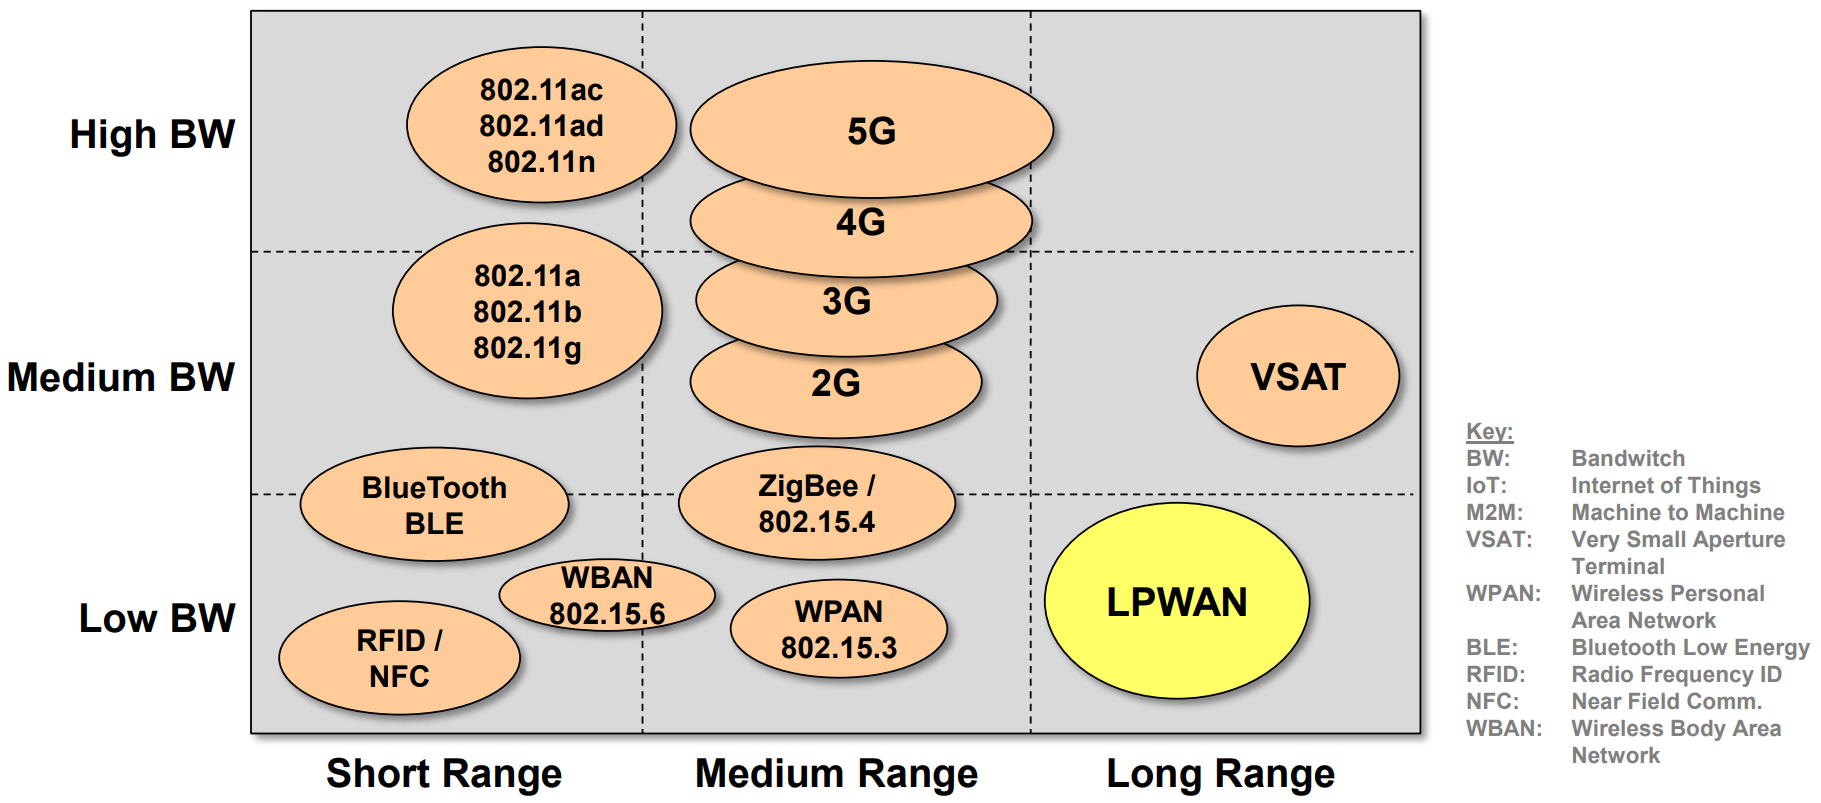
\includegraphics[width=\linewidth]{fig/lpwan_gap.png}
\vspace*{3mm}
\caption{Target of LPWAN technologies \cite{peteregli_lpwan}.}
\label{fig:lpwan_gap}
\end{figure}

There are several emerging and competing LPWAN technologies. LoRa, Sigfox, NB-IoT and LTE-M are commonly used, well-known LPWAN technologies \cite{7815384}. LoRa and Sigfox use license free ISM frequency bands while NB-IoT and LTE-M use licensed frequency bands which brings extra cost \cite{7815384}. Both LoRa and Sigfox are known for ultra-low power consumption and resilience to interference. While NB-IoT and LTE-M are promoted for higher data rate. LoRa has open standard MAC protocol called LoRaWAN. LoRaWAN and Sigfox MAC protocols are based on pure ALOHA medium access \cite{Abramson:1970:ASA:1478462.1478502}. LoRaWAN networks can be deployed as a private network like WiFi. However, Sigfox and NB-IoT are only available with operator contract \cite{7815384}. Number of messages that Sigfox end device can send in a day is limited to 140 packets for uplink and just 4 packets for downlink \cite{sigfox}. Also, Sigfox packet payload size is limited to 12 bytes for uplink and 8 bytes for downlink. However, LoRa supports up to 243 bytes payload size and NB-IoT supports up to 1600 bytes payload size. Sigfox maximum data rate is 100 bps, on the other hand maximum data rate for LoRa and NB-IoT are 50 kbps and 200 kbps respectively \cite{7815384}.

\begin{figure}[h]
\centering
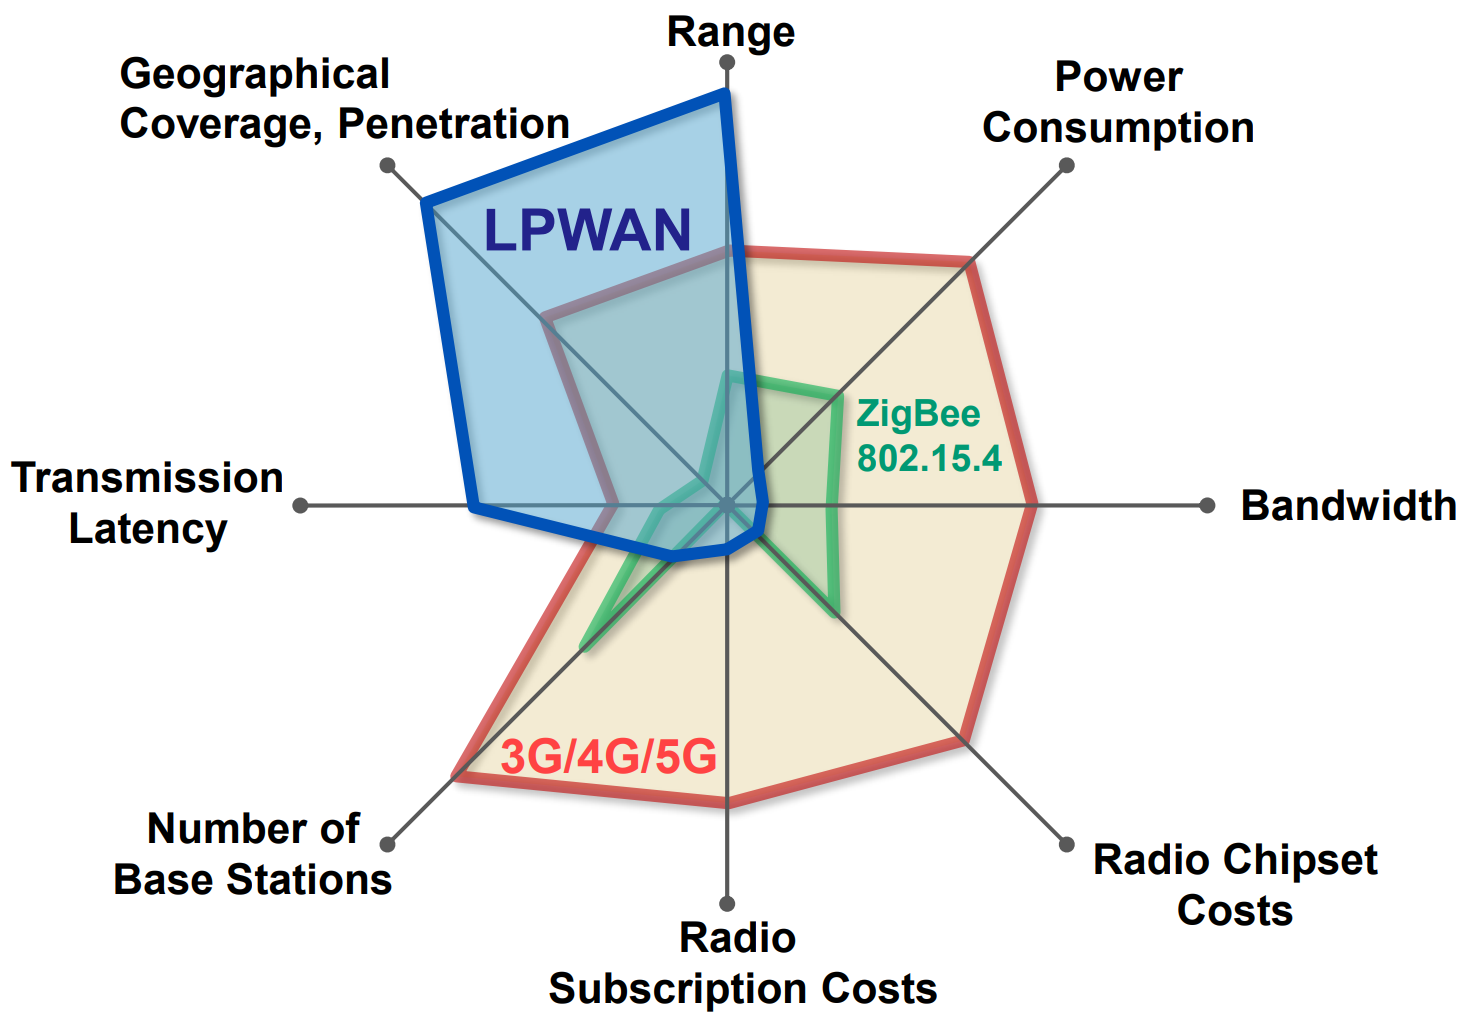
\includegraphics[width=0.8\linewidth]{fig/lpwan_features.png}
\vspace*{5mm}
\caption{Characteristics of LPWAN technologies \cite{peteregli_lpwan}.}
\label{fig:lpwan_features}
\end{figure}

LoRa can adjust data rate by spreading symbols within a fixed channel bandwidth. This enables tradeoff between receive sensitivity and air time of transmission \cite{7803607}. LoRa supports 6 different spreading factor (SF) options. Simultaneous same spreading factor transmissions are prone to collision, however, different spreading factor transmissions in the same channel are orthogonal to each other. Thus, spreading factor assignment is crucial for overall network performance.

\section{Contribution}
In this work, a LoRa discrete event simulator is developed from scratch to study the performance of various LoRa spreading factor assignment strategies. The tool is capable of simulating multiple node and multiple gateway LoRaWAN networks. The simulation tool can be fed with input parameters such as number of gateways, number of nodes, network radius, packet size, packet generation rate and with these inputs the tool produces simulation results such as total number of generated packets, number of successfully received packets, number of interfered packets, number of under sensitivity packets, network packet delivery ratio percentage, network throughput, total transmit energy consumption. 

In this work, first, spreading factor assignment challenge for both single gateway and multiple gateway networks are described. It is shown how spreading factor assignment effects collisions and network performance. Then, an avoidance mechanism is proposed to decrease number of collisions. A machine learning based spreading factor assignment approach is proposed. Support Vector Machine (SVM) and Decision Tree Classifier (DTC) machine learning methods are employed and the introduced schemes are called as smart spreading factor assignment schemes. Smart spreading factor schemes are integrated into the simulation tool. The performance of the smart schemes is compared with the performance of the lowest spreading factor assignment scheme. It is shown that the proposed smart spreading factor assignment schemes give promising results.

\section{Organization of the Thesis}
This thesis is organized as follows:

Chapter \ref{ch:lora_lorawan} provides background information about LoRa and LoRaWAN. First, LoRa spreading factor and spreading factor assignment issue is covered. Then, LoRaWAN architecture and LoRaWAN network entities are explained.

Other recent related works are summarized in Chapter \ref{ch:related_works}.

Chapter \ref{ch:proposed_technique} describes the proposed smart spreading factor assignment techniques. Two machine learning method is utilized to solve spreading factor assignment issue described in Chapter \ref{ch:lora_lorawan}.

Simulation environment is described in Chapter \ref{ch:simulation_environment}. First, employed link model and interference model are explained. Then, software structure of the simulation tool is described.

Simulation results are shown and discussed in Chapter \ref{ch:simulation_results}. Foremost, single gateway network topology simulation results are shown. Then, multiple gateway network topology simulation results alongside with smart spreading factor schemes simulation results are shown. 

Finally, Chapter \ref{ch:conclusion} concludes the thesis by giving future directions.
